\chapter{Risultati Empirici}
Dall'analisi dei valori notiamo che le migliori soluzioni escludono, per la maggior parte, l'utilizzo di 10.000 kernel se non con un valore di OFFSET abbastanza alto e di conseguenza un KNN molto semplificato.
Contrariamente a quanto affermato nei paper, relativi ad entrambi i modelli, ROCKET e ROCKAD non hanno un efficienza così elevata.
Prendendo, infatti, in considerazione il dataset OPS\textunderscore SAT, in caso di un valore basso di STEP, o nel caso del dataset NASA prendendo un valore basso di OFFSET, riscontriamo un efficienza non ottimale.

Nella fase di test, su OPS\textunderscore SAT, non è stato possibile estrarre le metriche con un valore di STEP inferiore a 250, dato che portava ad un esecuzione che avrebbe richiesto troppo tempo per terminare.

Per osservare meglio l'andamento dei modelli in base al numero di kernel, riportiamo le misurazioni rilevate dai test nei grafici in Figura \ref{fig:grafico_f1_ROCKET_OPS_SAT} e Figura \ref{fig:grafico_f1_ROCKAD_OPS_SAT}, che mettono in relazione il numero di kernel e la metrica F1.
\begin{figure}[!ht]
    \centering
    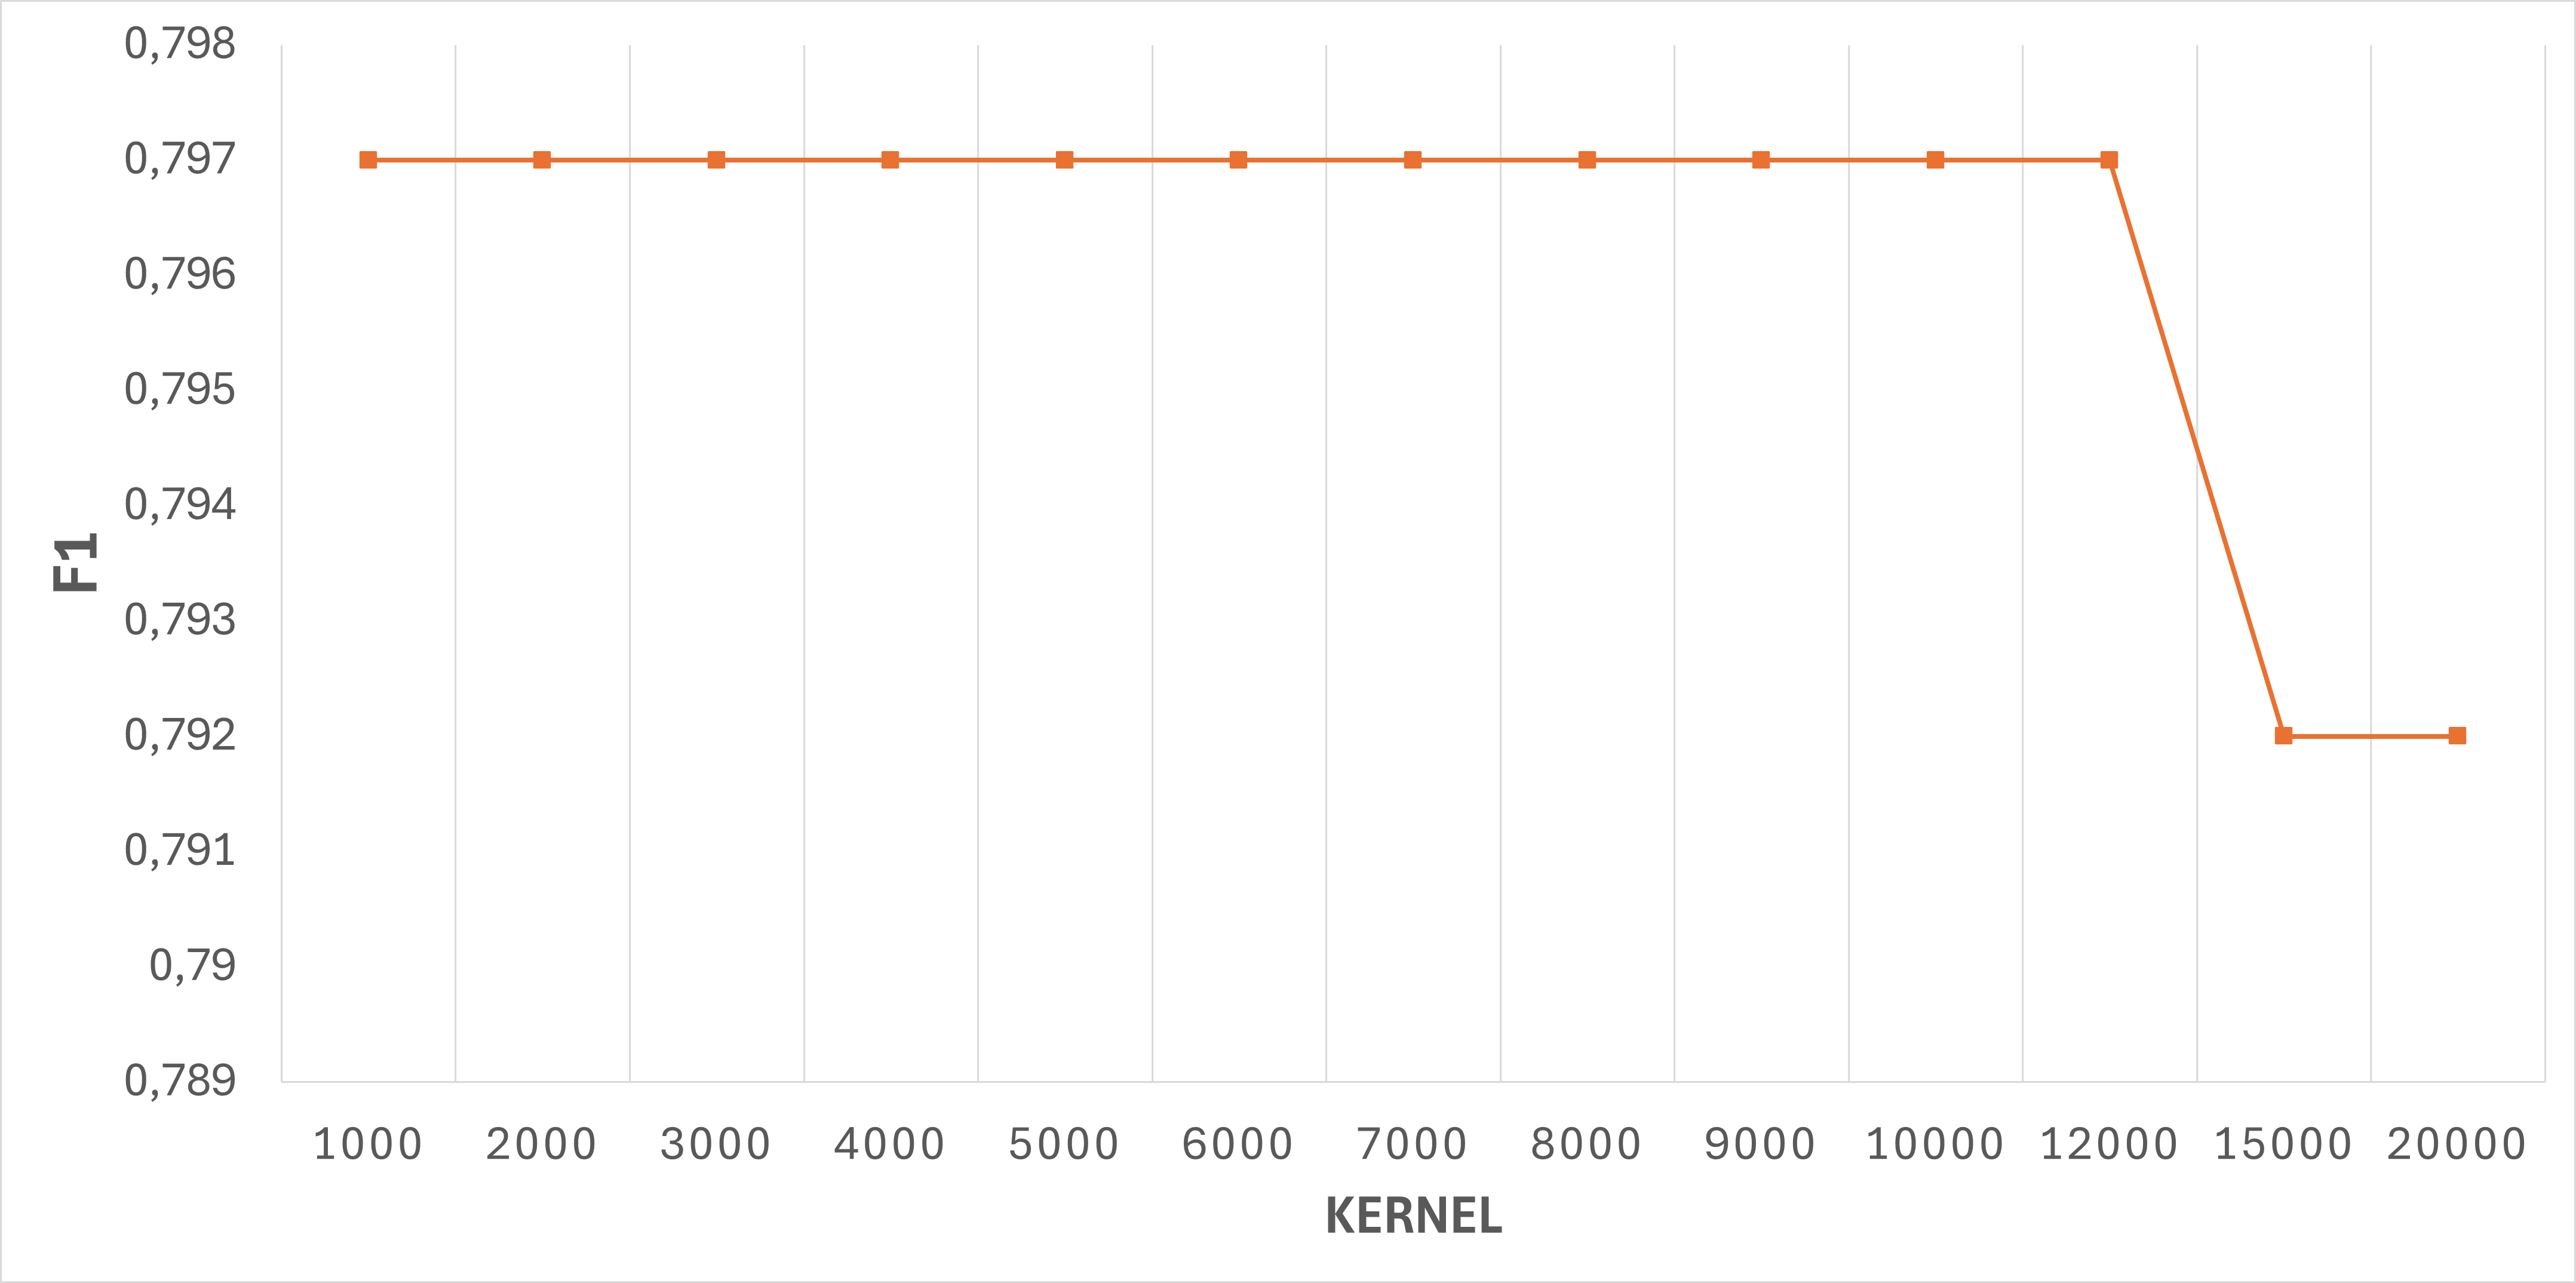
\includegraphics[width=0.9\linewidth]{images//Capitolo7/GraficoF1_ROCKET_OPS_SAT.png}
    \caption{Relazione tra F1 e Numero di Kernel - ROCKET}
    \label{fig:grafico_f1_ROCKET_OPS_SAT}
\end{figure}
\pagebreak

\begin{figure}[!ht]
    \centering
    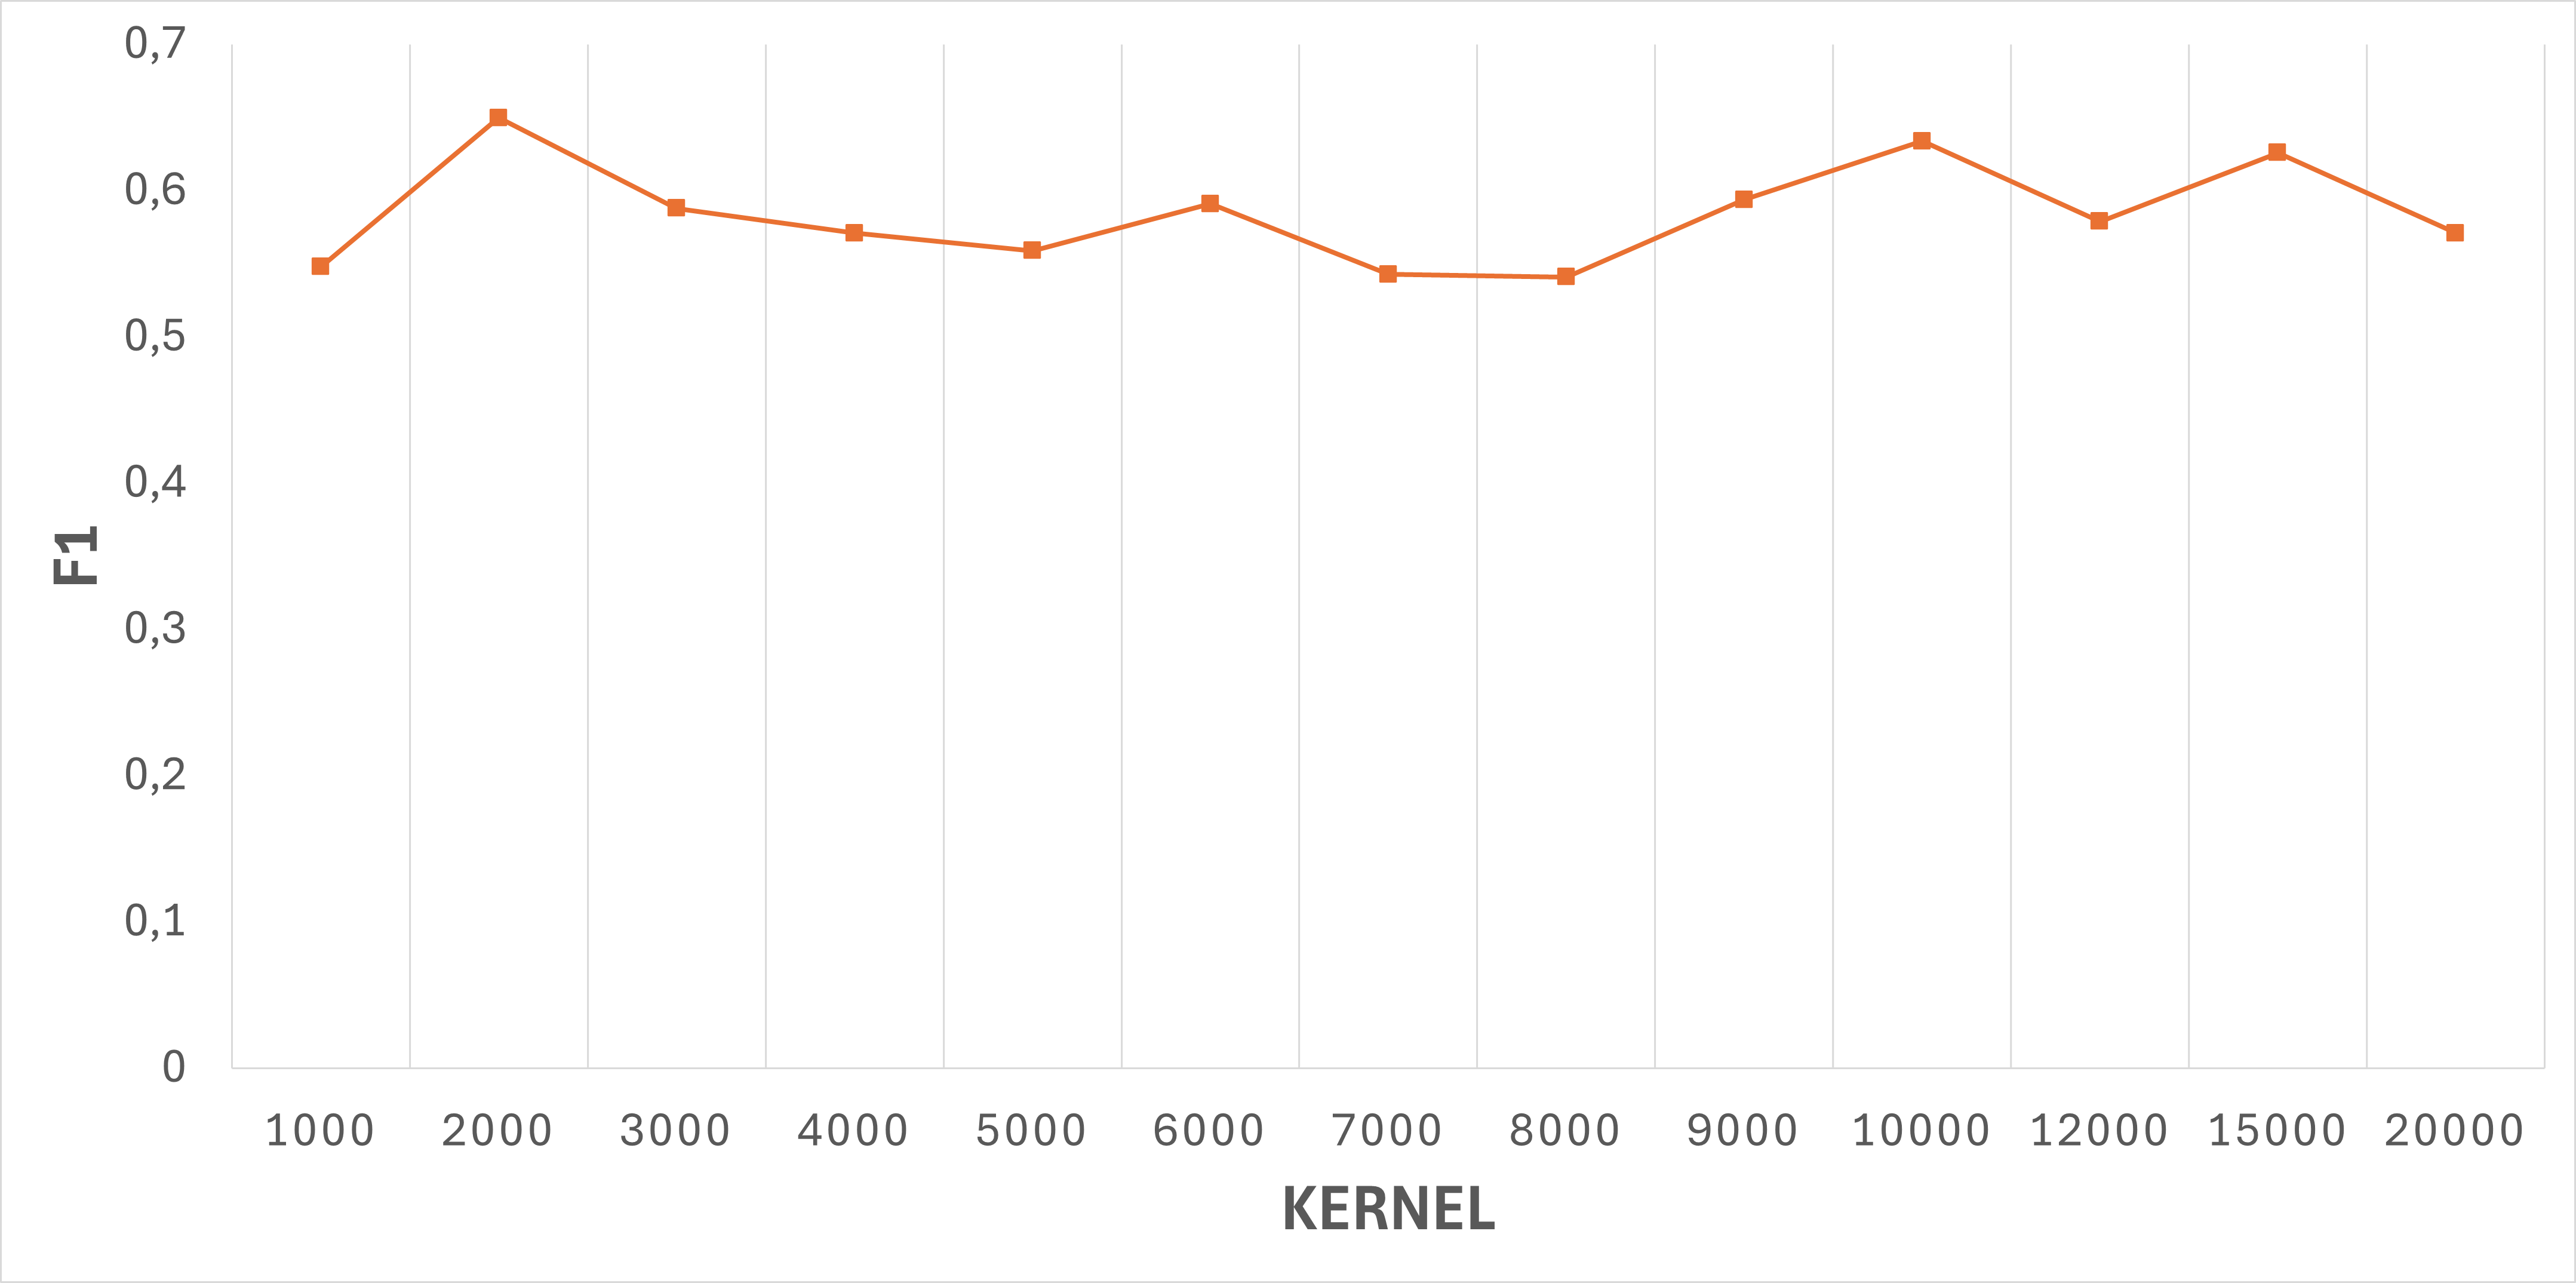
\includegraphics[width=0.9\linewidth]{images//Capitolo7/GraficoF1_ROCKAD_OPS_SAT.png}
    \caption{Relazione tra F1 e Numero di Kernel - ROCKAD}
    \label{fig:grafico_f1_ROCKAD_OPS_SAT}
\end{figure}

Oltre a tenere in considerazione l'F1, riportiamo in aggiunta, il tempo di esecuzione al variare del numero di kernel nel grafico in Figura \ref{fig:grafico_Tempo_ROCKET_OPS_SAT} per ROCKET e in quello in Figura \ref{fig:grafico_Tempo_ROCKAD_OPS_SAT} per ROCKAD.


\begin{figure}[!ht]
    \centering
    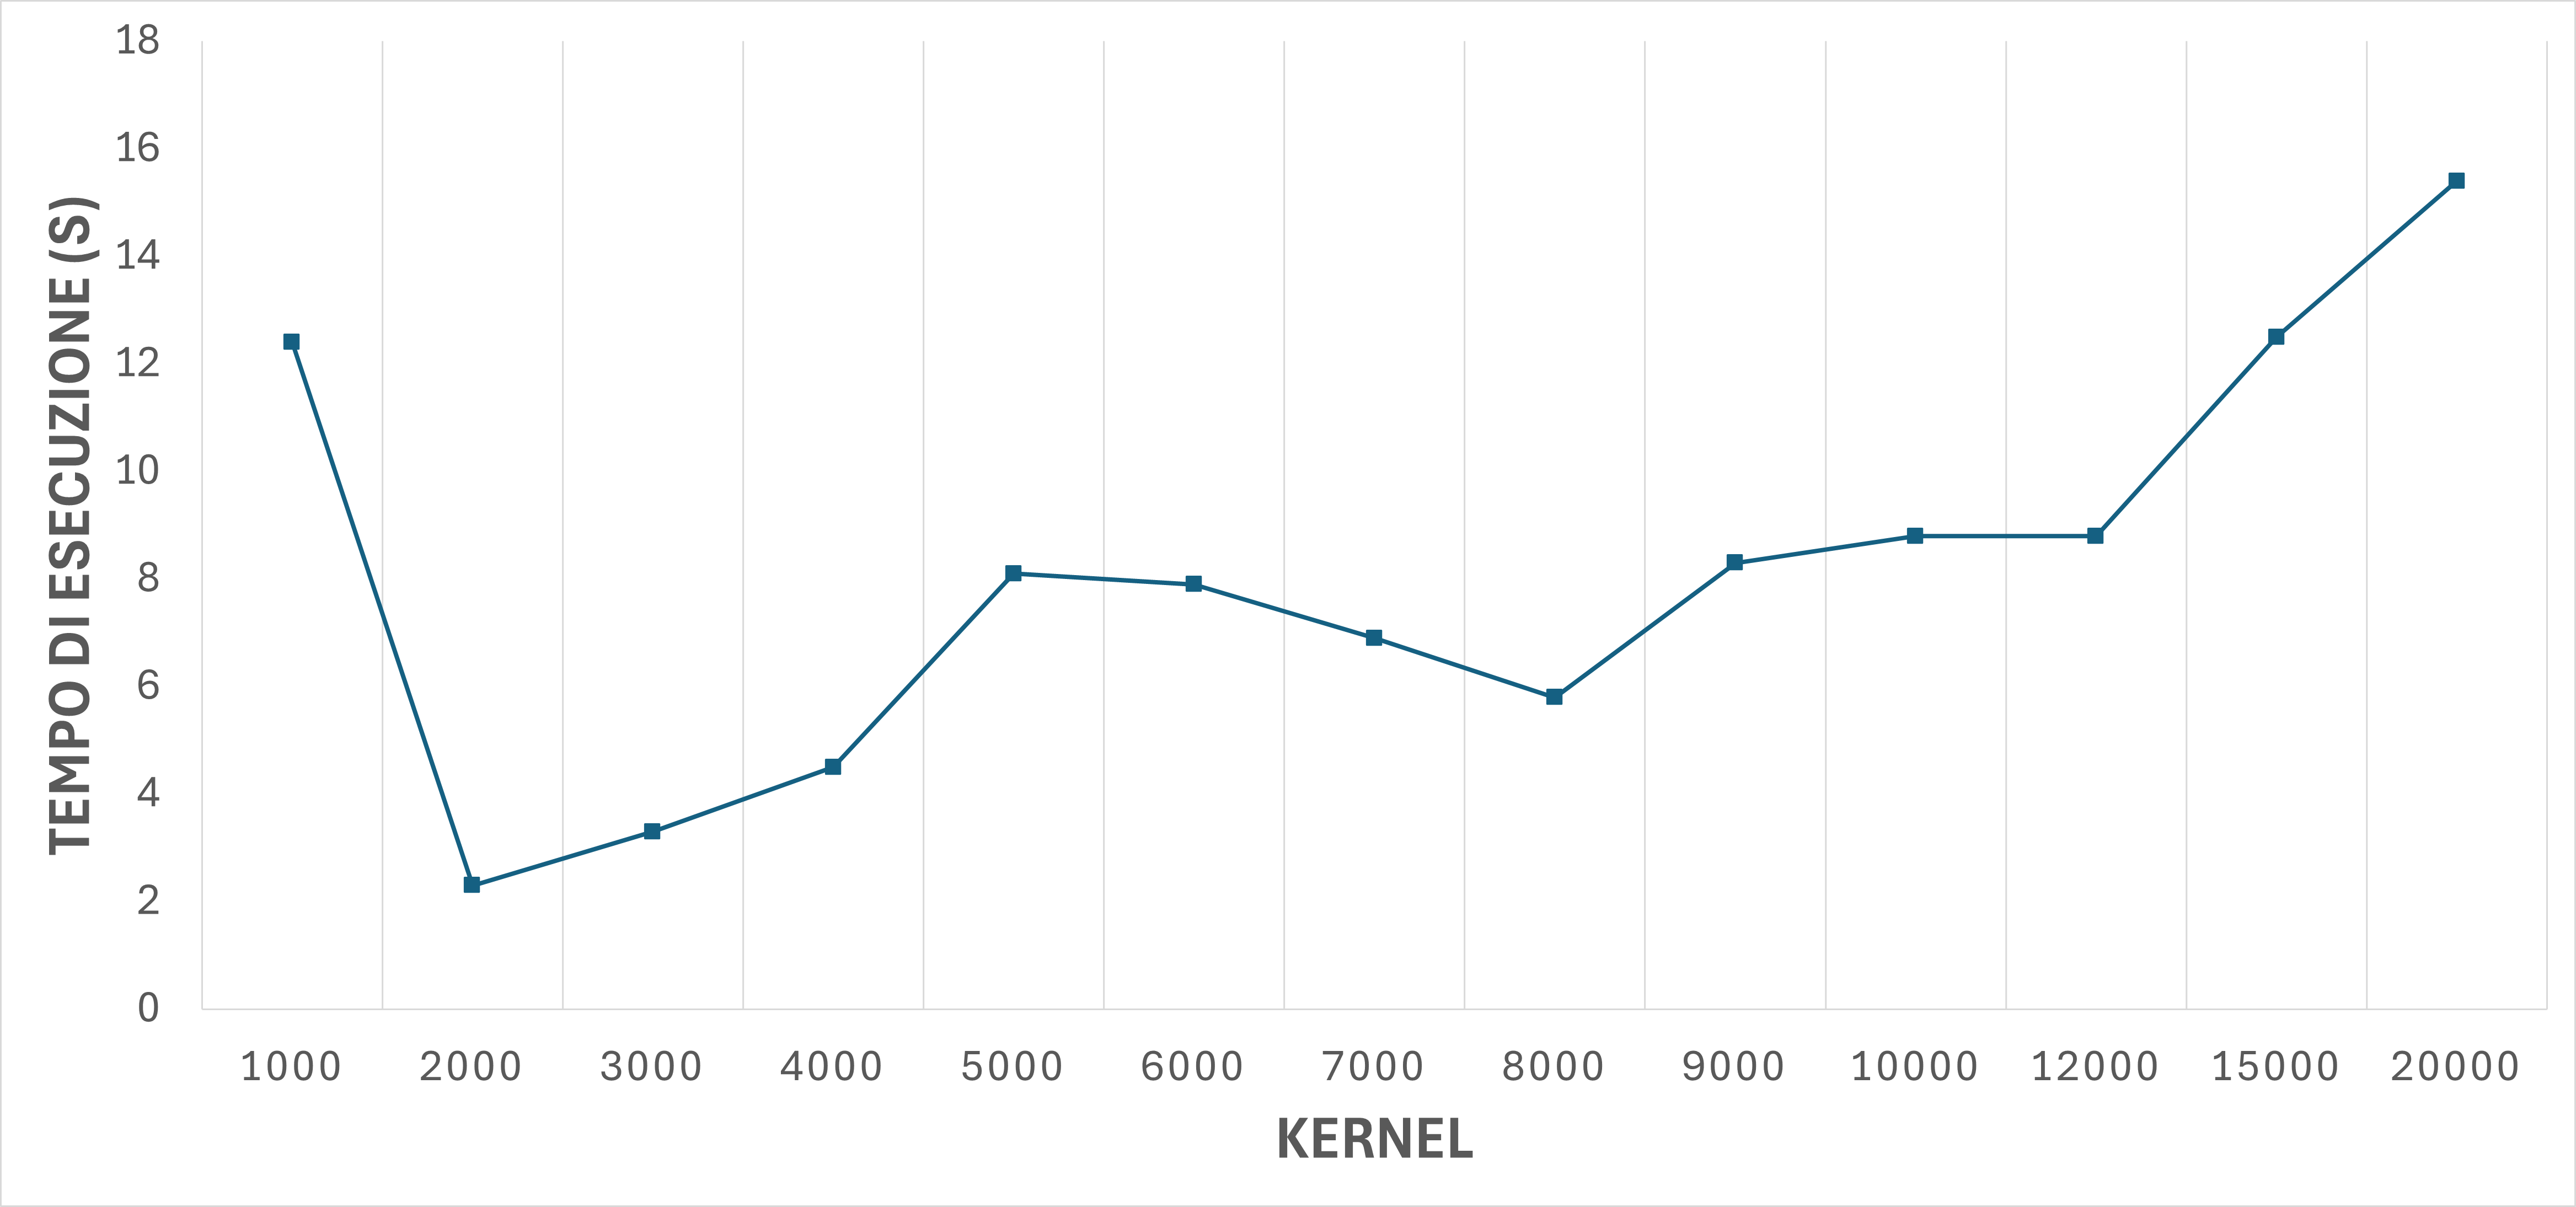
\includegraphics[width=0.9\linewidth]{images//Capitolo7/GraficoTempoEsecuzione_ROCKET_OPS_SAT.png}
    \caption{Relazione tra F1 e Numero di Kernel - ROCKET}
    \label{fig:grafico_Tempo_ROCKET_OPS_SAT}
\end{figure}

\begin{figure}[!ht]
    \centering
    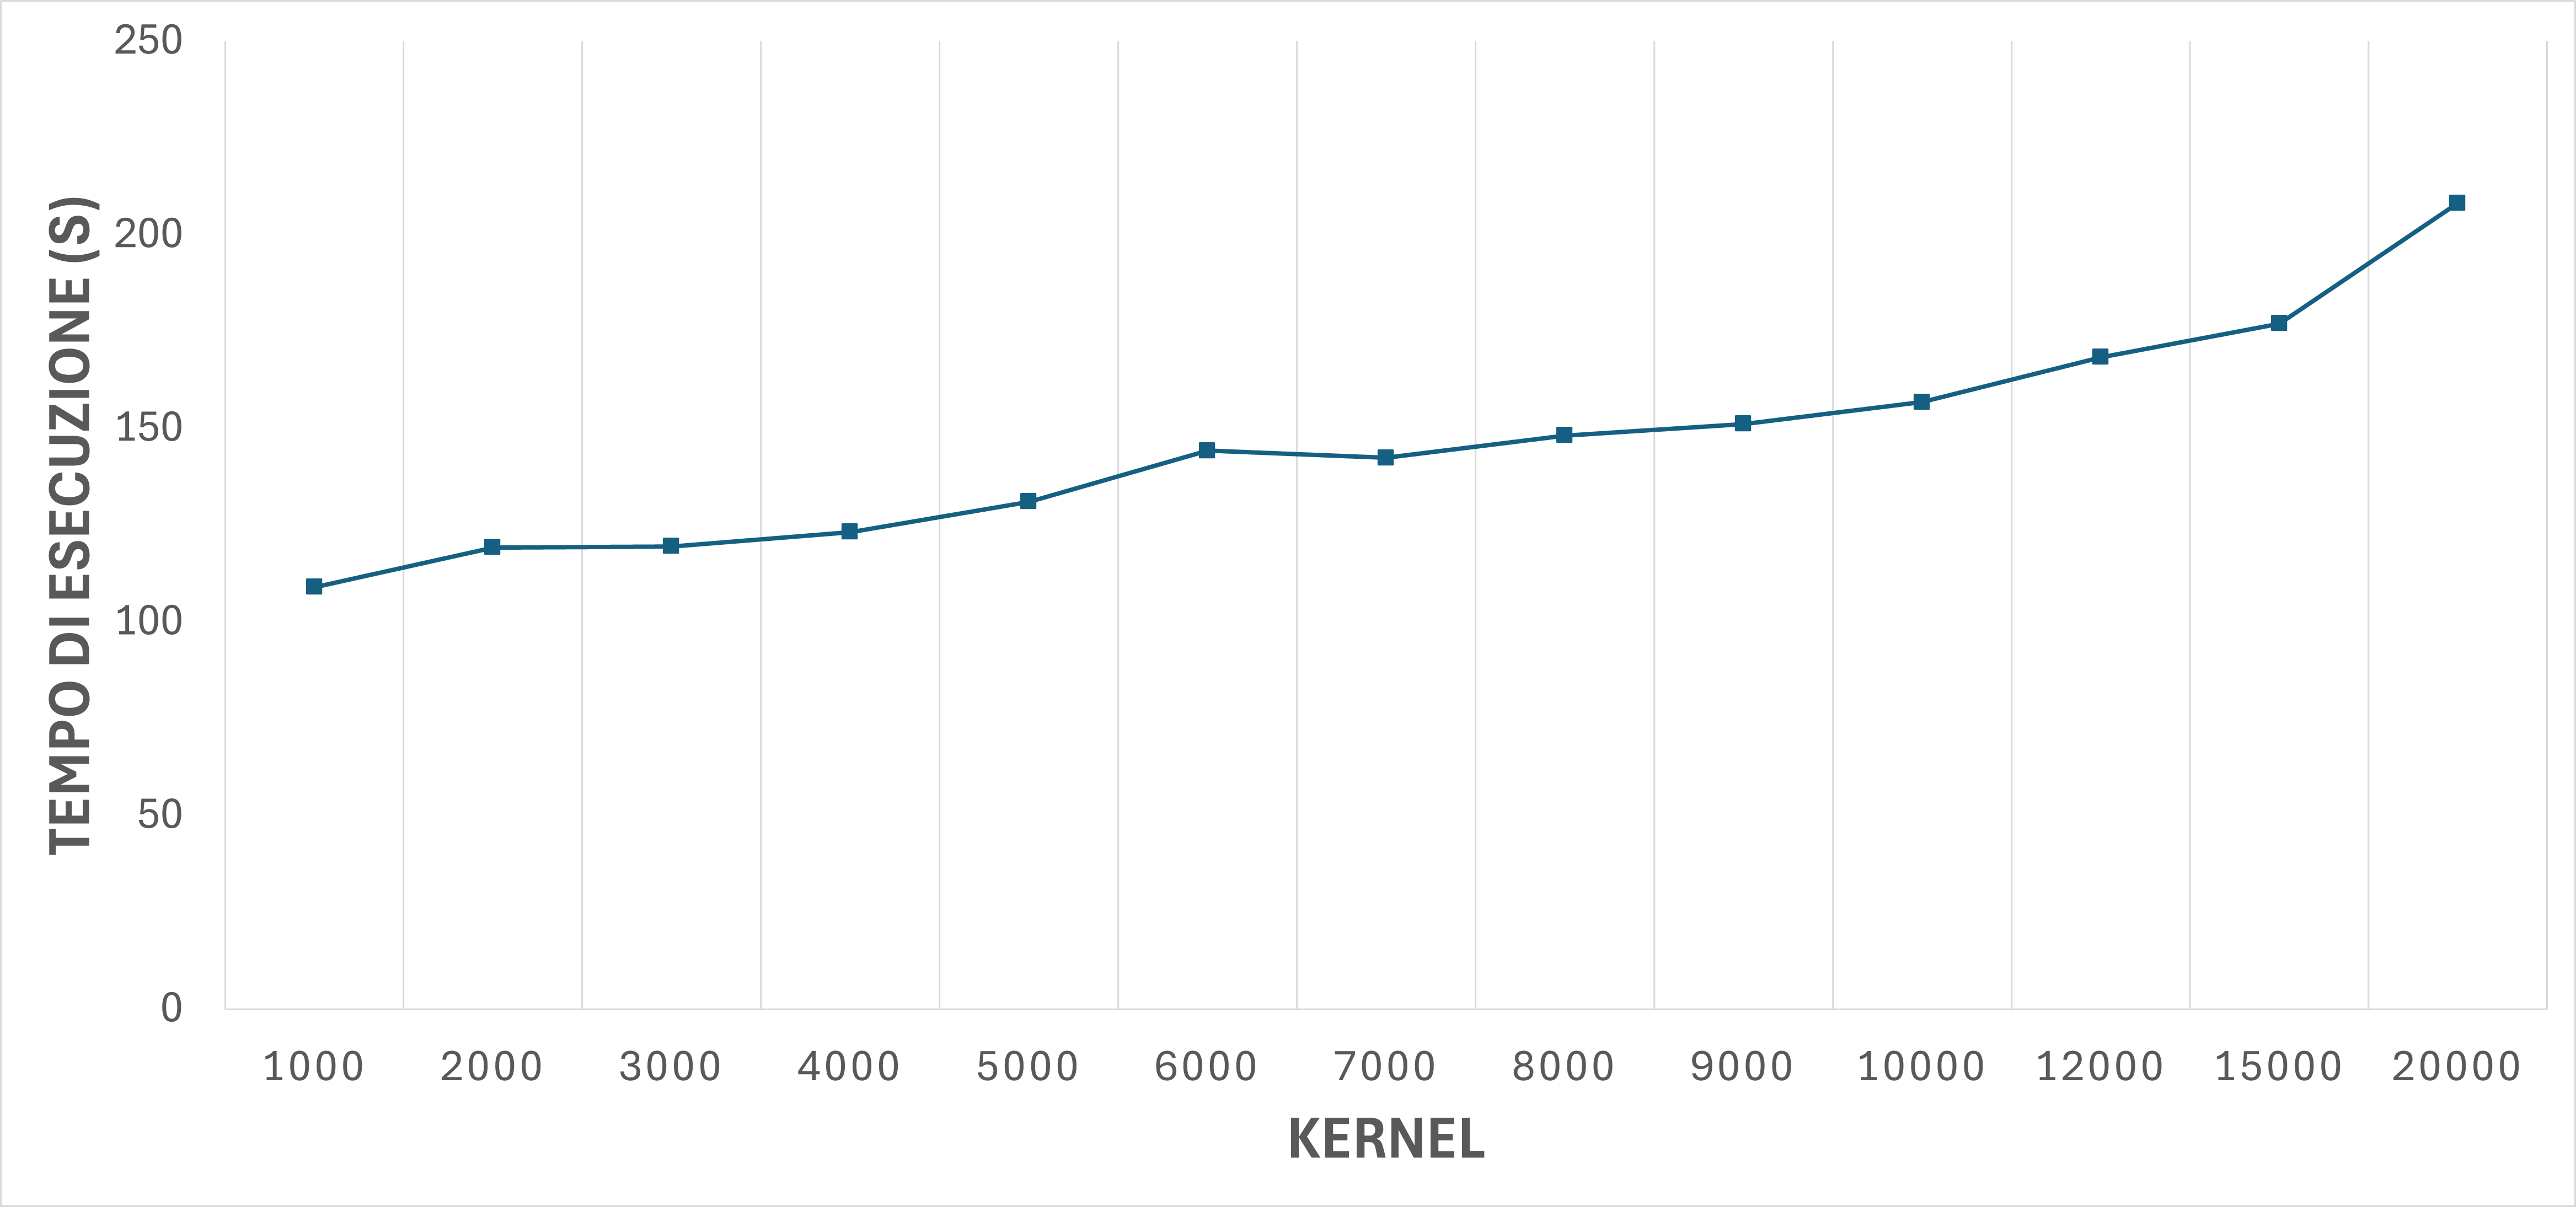
\includegraphics[width=0.9\linewidth]{images//Capitolo7/GraficoTempoEsecuzione_ROCKAD_OPS_SAT.png}
    \caption{Relazione tra F1 e Numero di Kernel - ROCKAD}
    \label{fig:grafico_Tempo_ROCKAD_OPS_SAT}
\end{figure}

Per ottenere questi risultati abbiamo utilizzato gli algoritmi o iperparametri migliori riscontrati nei test precedenti: per ROCKET il classificatore RidgeClassifierCV e per ROCKAD 10 estimatori.
\pagebreak

\section{Risultati Dataset NASA}

Per il dataset NASA, invece, questa situazione si verificava con un numero di kernel pari a 10.000 ed un valore di OFFSET inferiore a 50, questo valore di OFFSET portava con sé anche il problema di non poter aumentare il numero di nodi del KNN, per mancanza di vicini, data la struttura del dataset.

Relativamente alle metriche in questione, analizziamo il grafico in Figura \ref{fig:grafico_f1}, che mostra come cambia la metrica fondamentale, ossia l' F1, con l'aumentare dei kernel.
Nel caso di un numero di kernel pari a 1000 o 10.000 il valore di F1 è pressoché identico, mentre in tutti gli altri valori, la metrica diminuisce significativamente.
Da considerare nell'analisi dobbiamo evidenziare anche il tempo di esecuzione, come mostrato dal grafico nella Figura \ref{fig:grafico_Tempo}, che riporta i tempi di esecuzione dei vari valori dei kernel.

\begin{figure}[!ht]
    \centering
    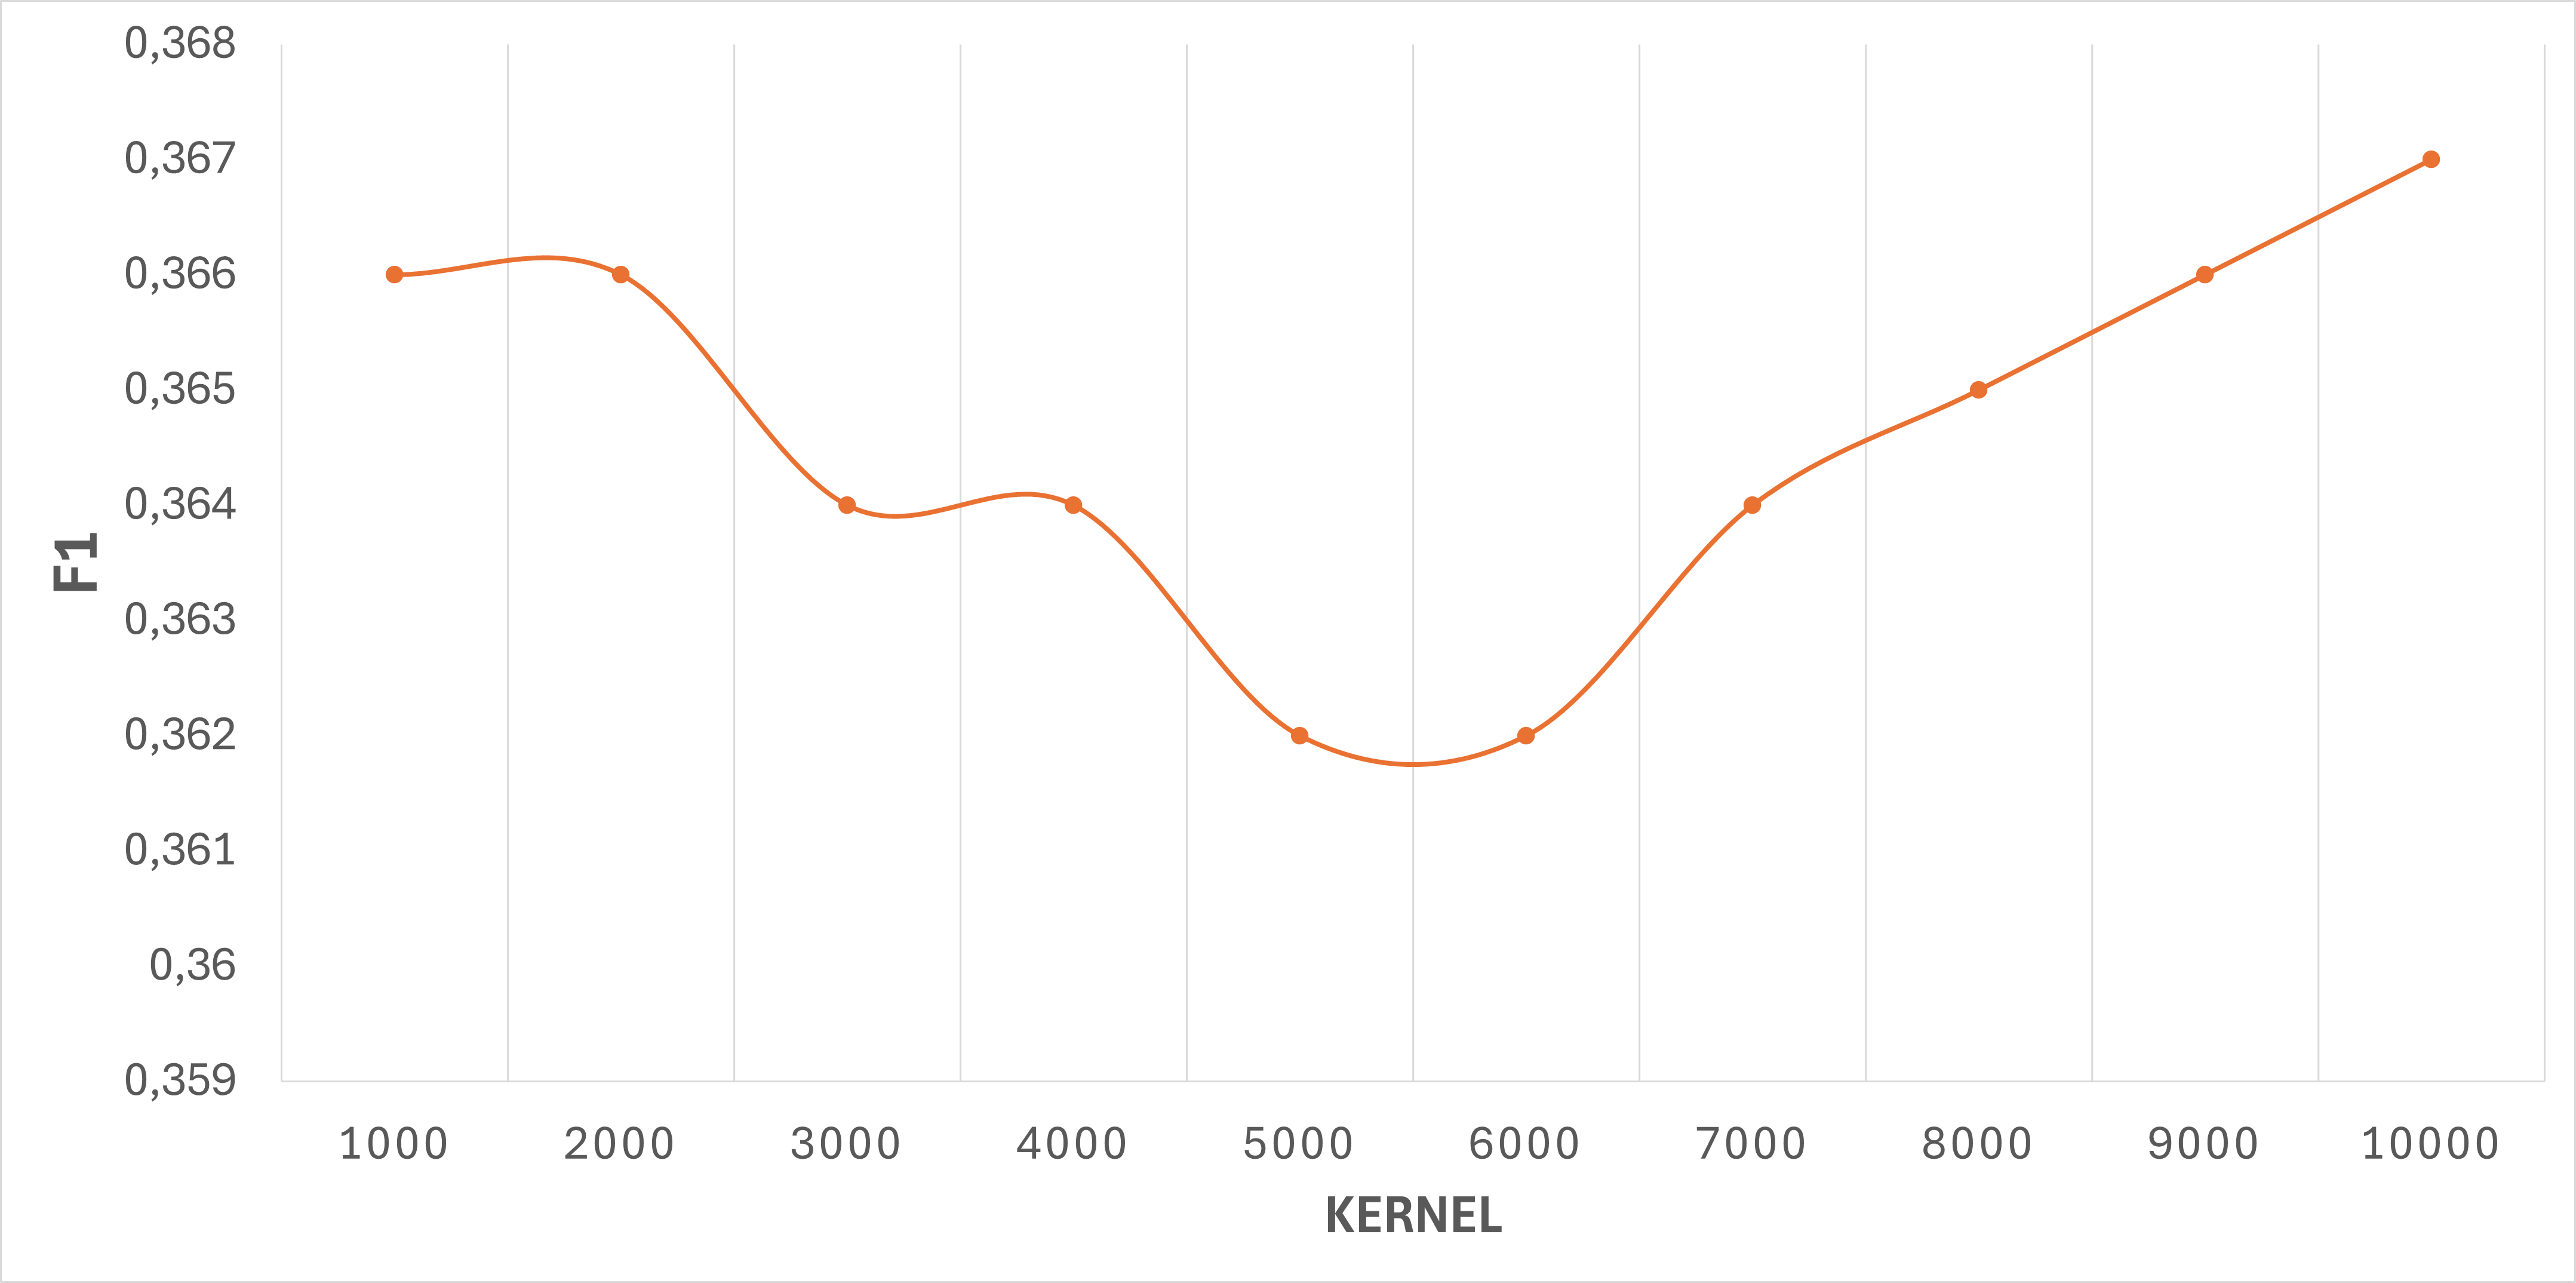
\includegraphics[width=0.9\linewidth]{images//Capitolo7/GraficoF1_ROCKET.png}
    \caption{Relazione tra F1 e Numero di Kernel}
    \label{fig:grafico_f1}
\end{figure}
\begin{figure}[!ht]
    \centering
    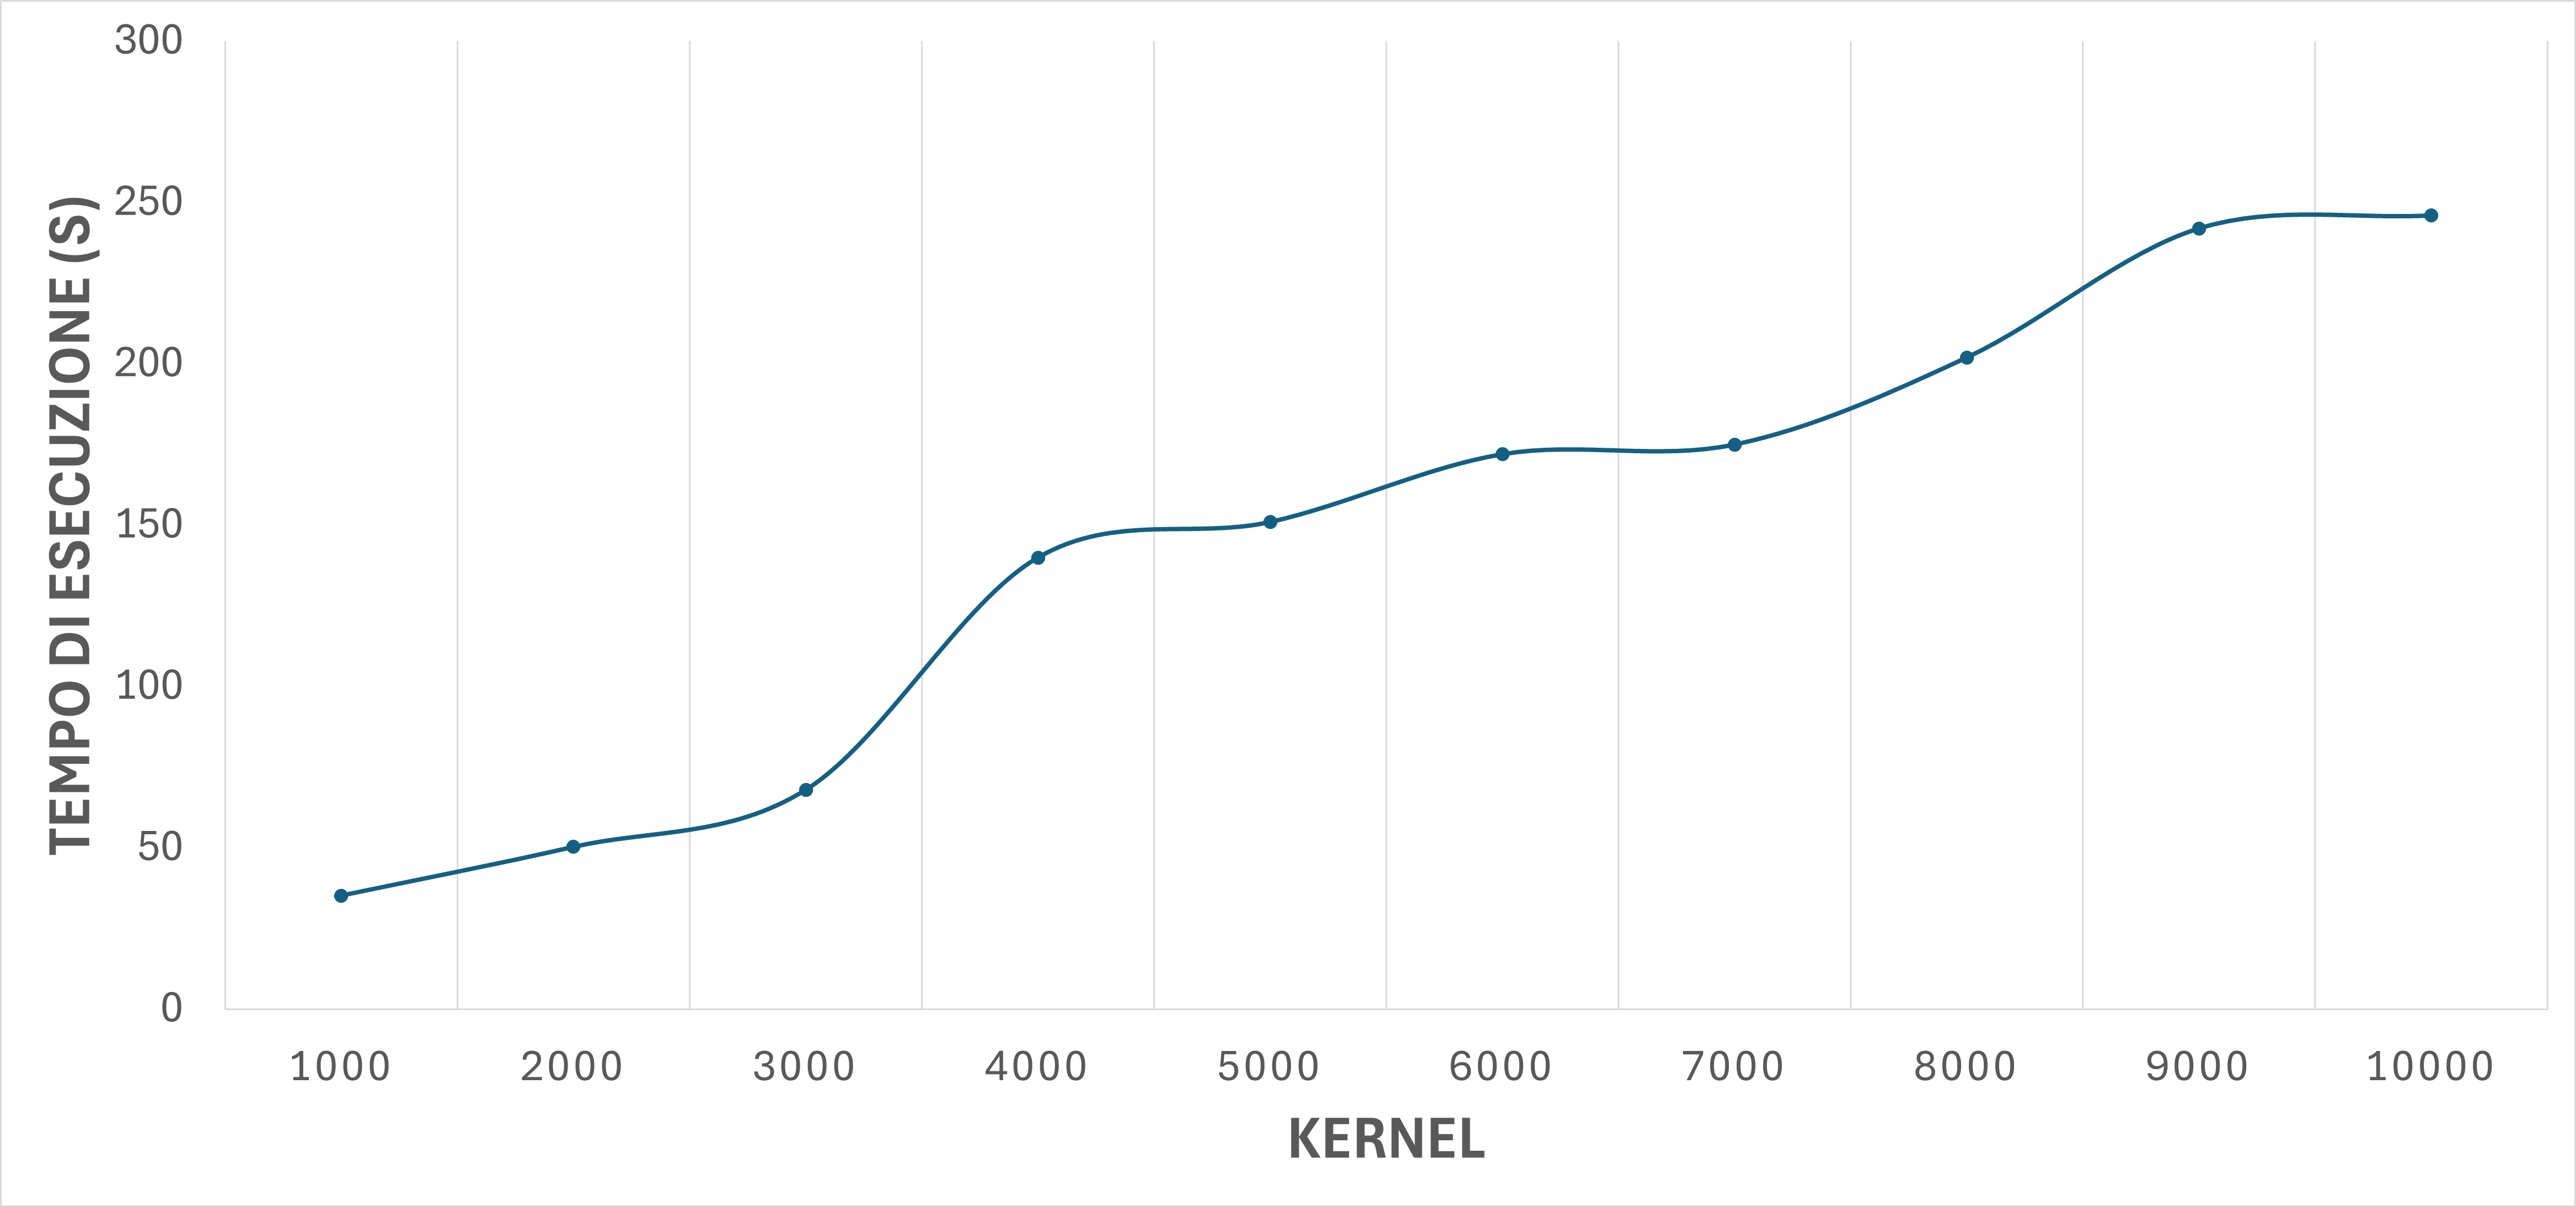
\includegraphics[width=0.9\linewidth]{images//Capitolo7/GraficoTempoEsecuzione_ROCKET.png}
    \caption{Relazione tra Tempi di Esecuzione e Numero di Kernel}
    \label{fig:grafico_Tempo}
\end{figure}
\pagebreak

Da questi grafici possiamo osservare come il tempo di esecuzione aumenti in maniera significativa all'aumentare del numero di kernel, lasciando invariati tutti gli altri parametri. Da questo, evidenziamo meglio che la scelta migliore per il numero di kernel, a parità di valore di F1, è indirizzata verso un valore pari a 1000, dove abbiamo un tempo di esecuzione quasi 7 volte minore rispetto a 10.000. 

Il problema che abbiamo nell'uso di ROCKET, soprattutto su NASA, è proprio quello evidenziato sopra, dato che fissando STEP a 250 l'algoritmo funziona senza troppi problemi e ad una velocità accettabile, ma al diminuire di questo valore il numero di caratteristiche aumenta esponenzialmente portando ad impiegare troppo tempo per fare training e test, non riuscendo a concludere la classificazione. 

Questa riflessione ci permette di capire che il collo di bottiglia di questa metodologia non è direttamente l'applicazione di ROCKET, ma la consecutiva applicazione di un algoritmo di classificazione, che avendo una grande quantità di features, non riesce a gestire in tempi normali.

In merito a ROCKAD, l'analisi della metrica F1 con un numero di kernel variabile tra 1000 e 10.000 è esposta nel grafico in Figura \ref{fig:grafico_f1_ROCKAD}.
Queste misurazioni sono state estratte mantenendo fissati il numero di n\textunderscore neighbors a 2 e OFFSET a 50; notiamo che questo ha un andamento diverso da quanto visto per ROCKET, portando a premiare un numero di kernel compreso tra 3000 e 5000, dove riscontriamo valori più alti di F1.

Il grafico è stato proposto con questi parametri a causa dei problemi relativi ai tempi di esecuzione, infatti nella Tabella \ref{tab:NASA_Posticipato} possiamo vedere come i parametri migliori hanno un OFFSET uguale a 30, ma provando l'esecuzione con quest'ultimo valore, l'algoritmo non terminava in tempi normali.
Infatti a conferma di quanto appena detto, come possiamo vedere dal grafico in Figura \ref{fig:grafico_tempo_ROCKAD}, i tempi di esecuzione, aumentano molto rapidamente fino ad arrivare, nel nostro caso, a più di dieci minuti; questo è stato paragonato con i valori di F1.

\begin{figure}[!ht]
    \centering
    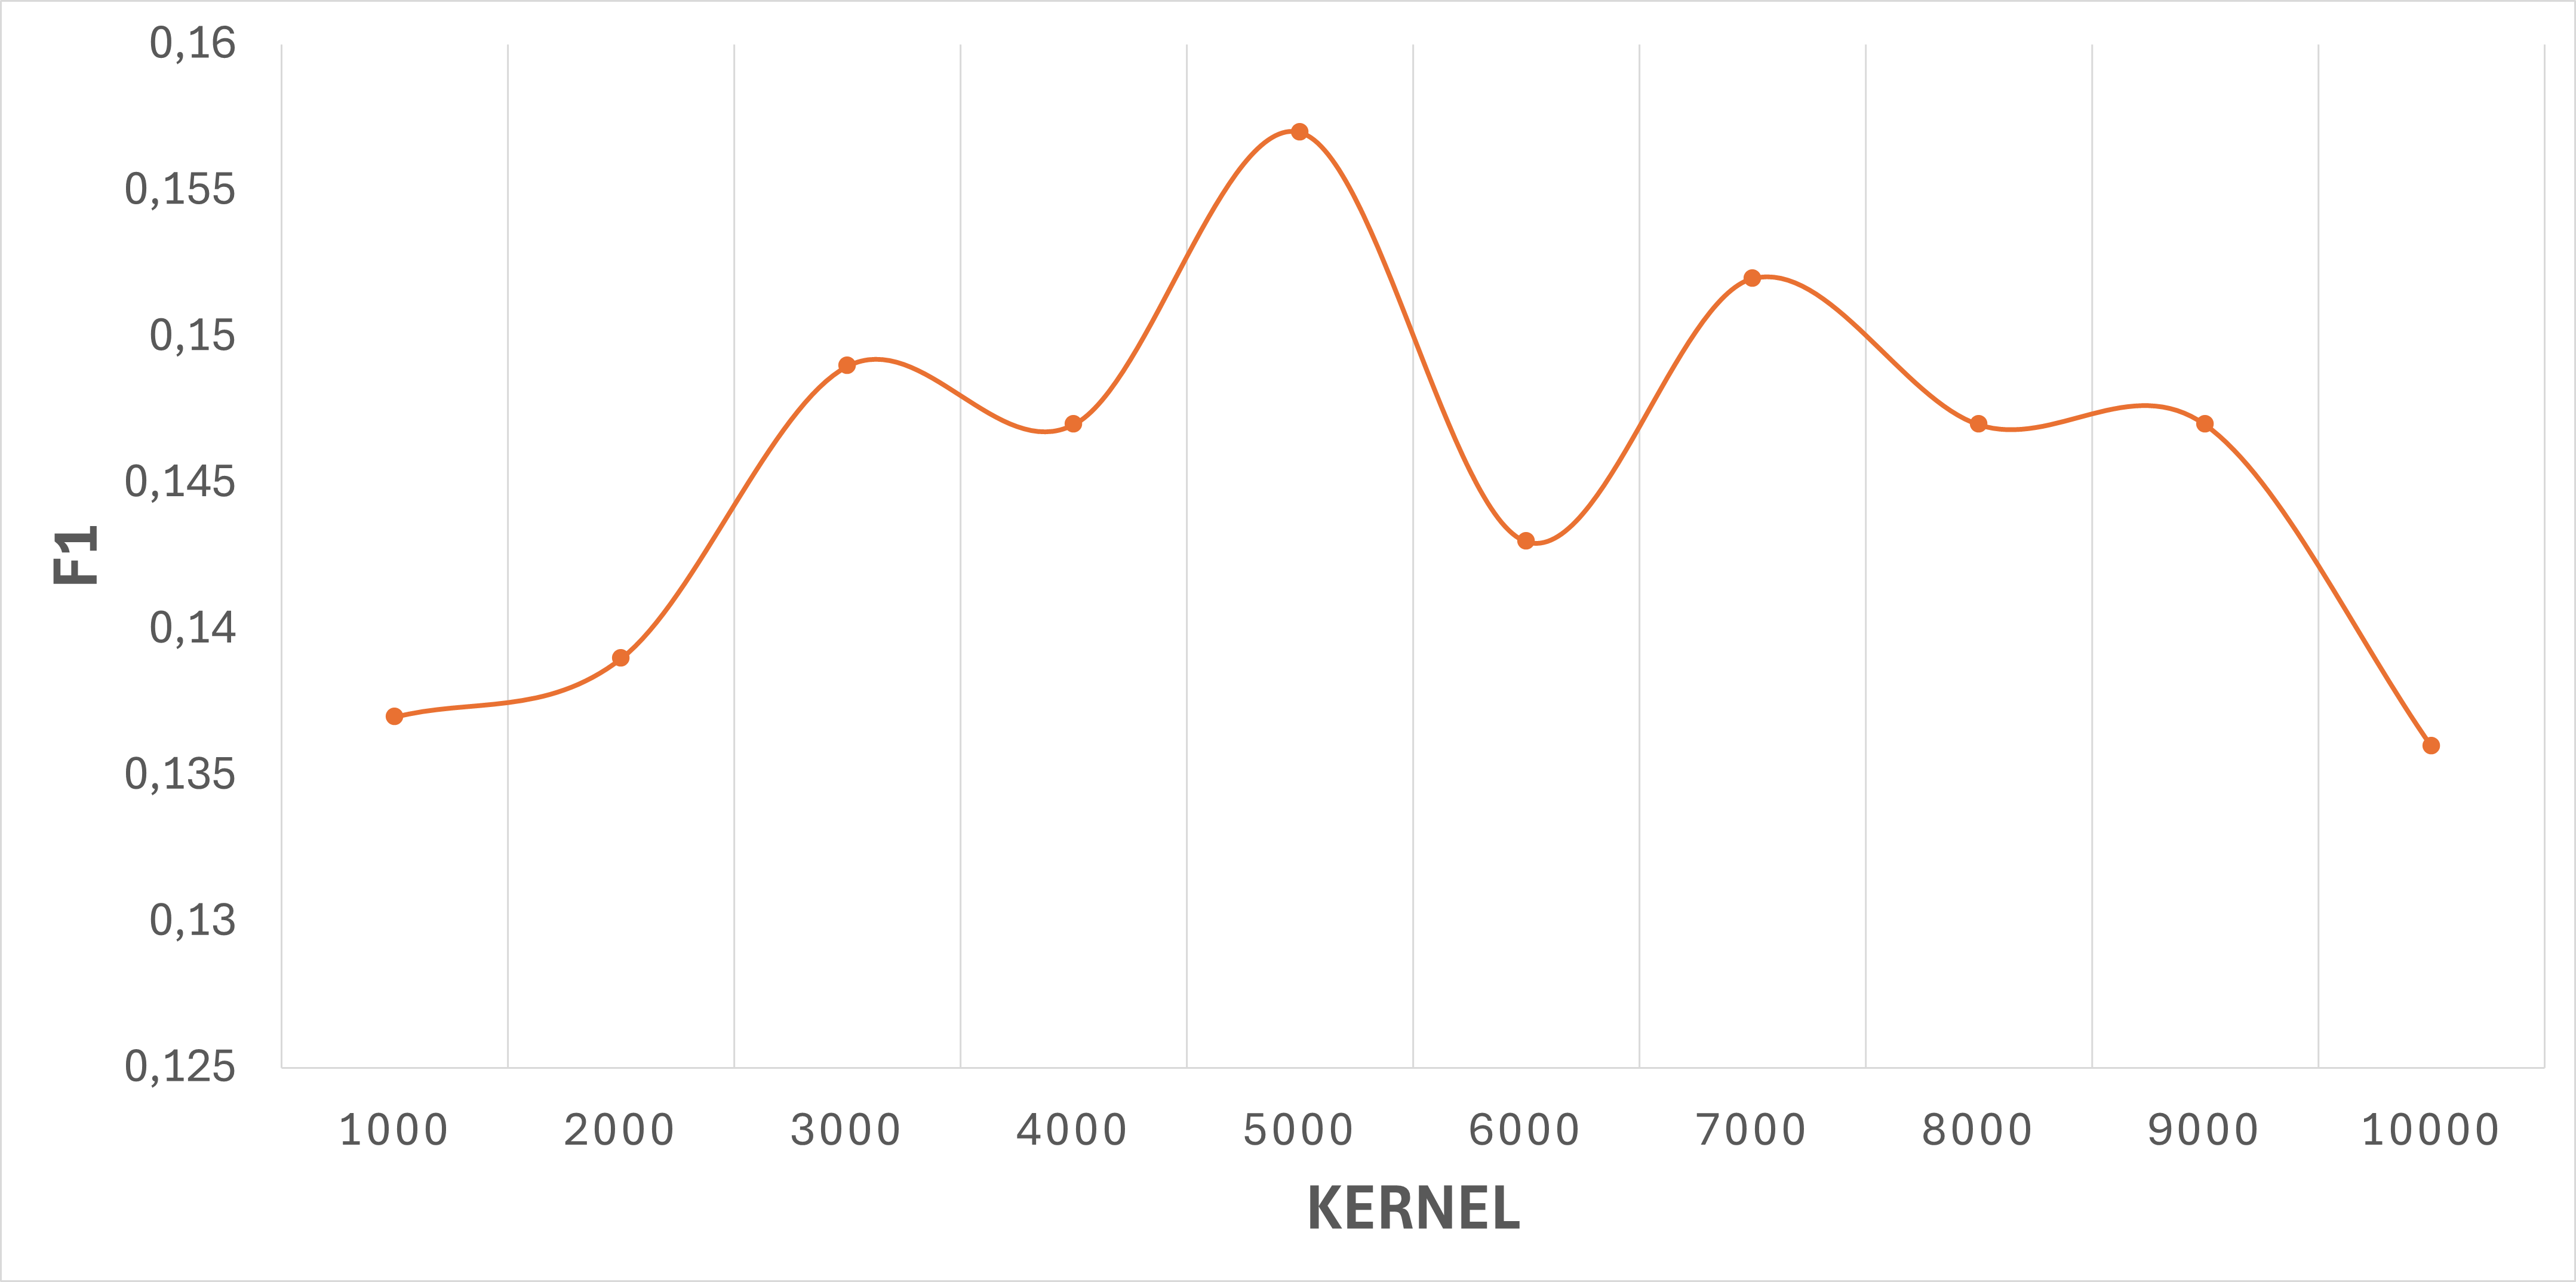
\includegraphics[width=0.9\linewidth]{images//Capitolo7/GraficoF1_ROCKAD.png}
    \caption{Relazione tra F1 e Numero di Kernel}
    \label{fig:grafico_f1_ROCKAD}
\end{figure}

\begin{figure}[!ht]
    \centering
    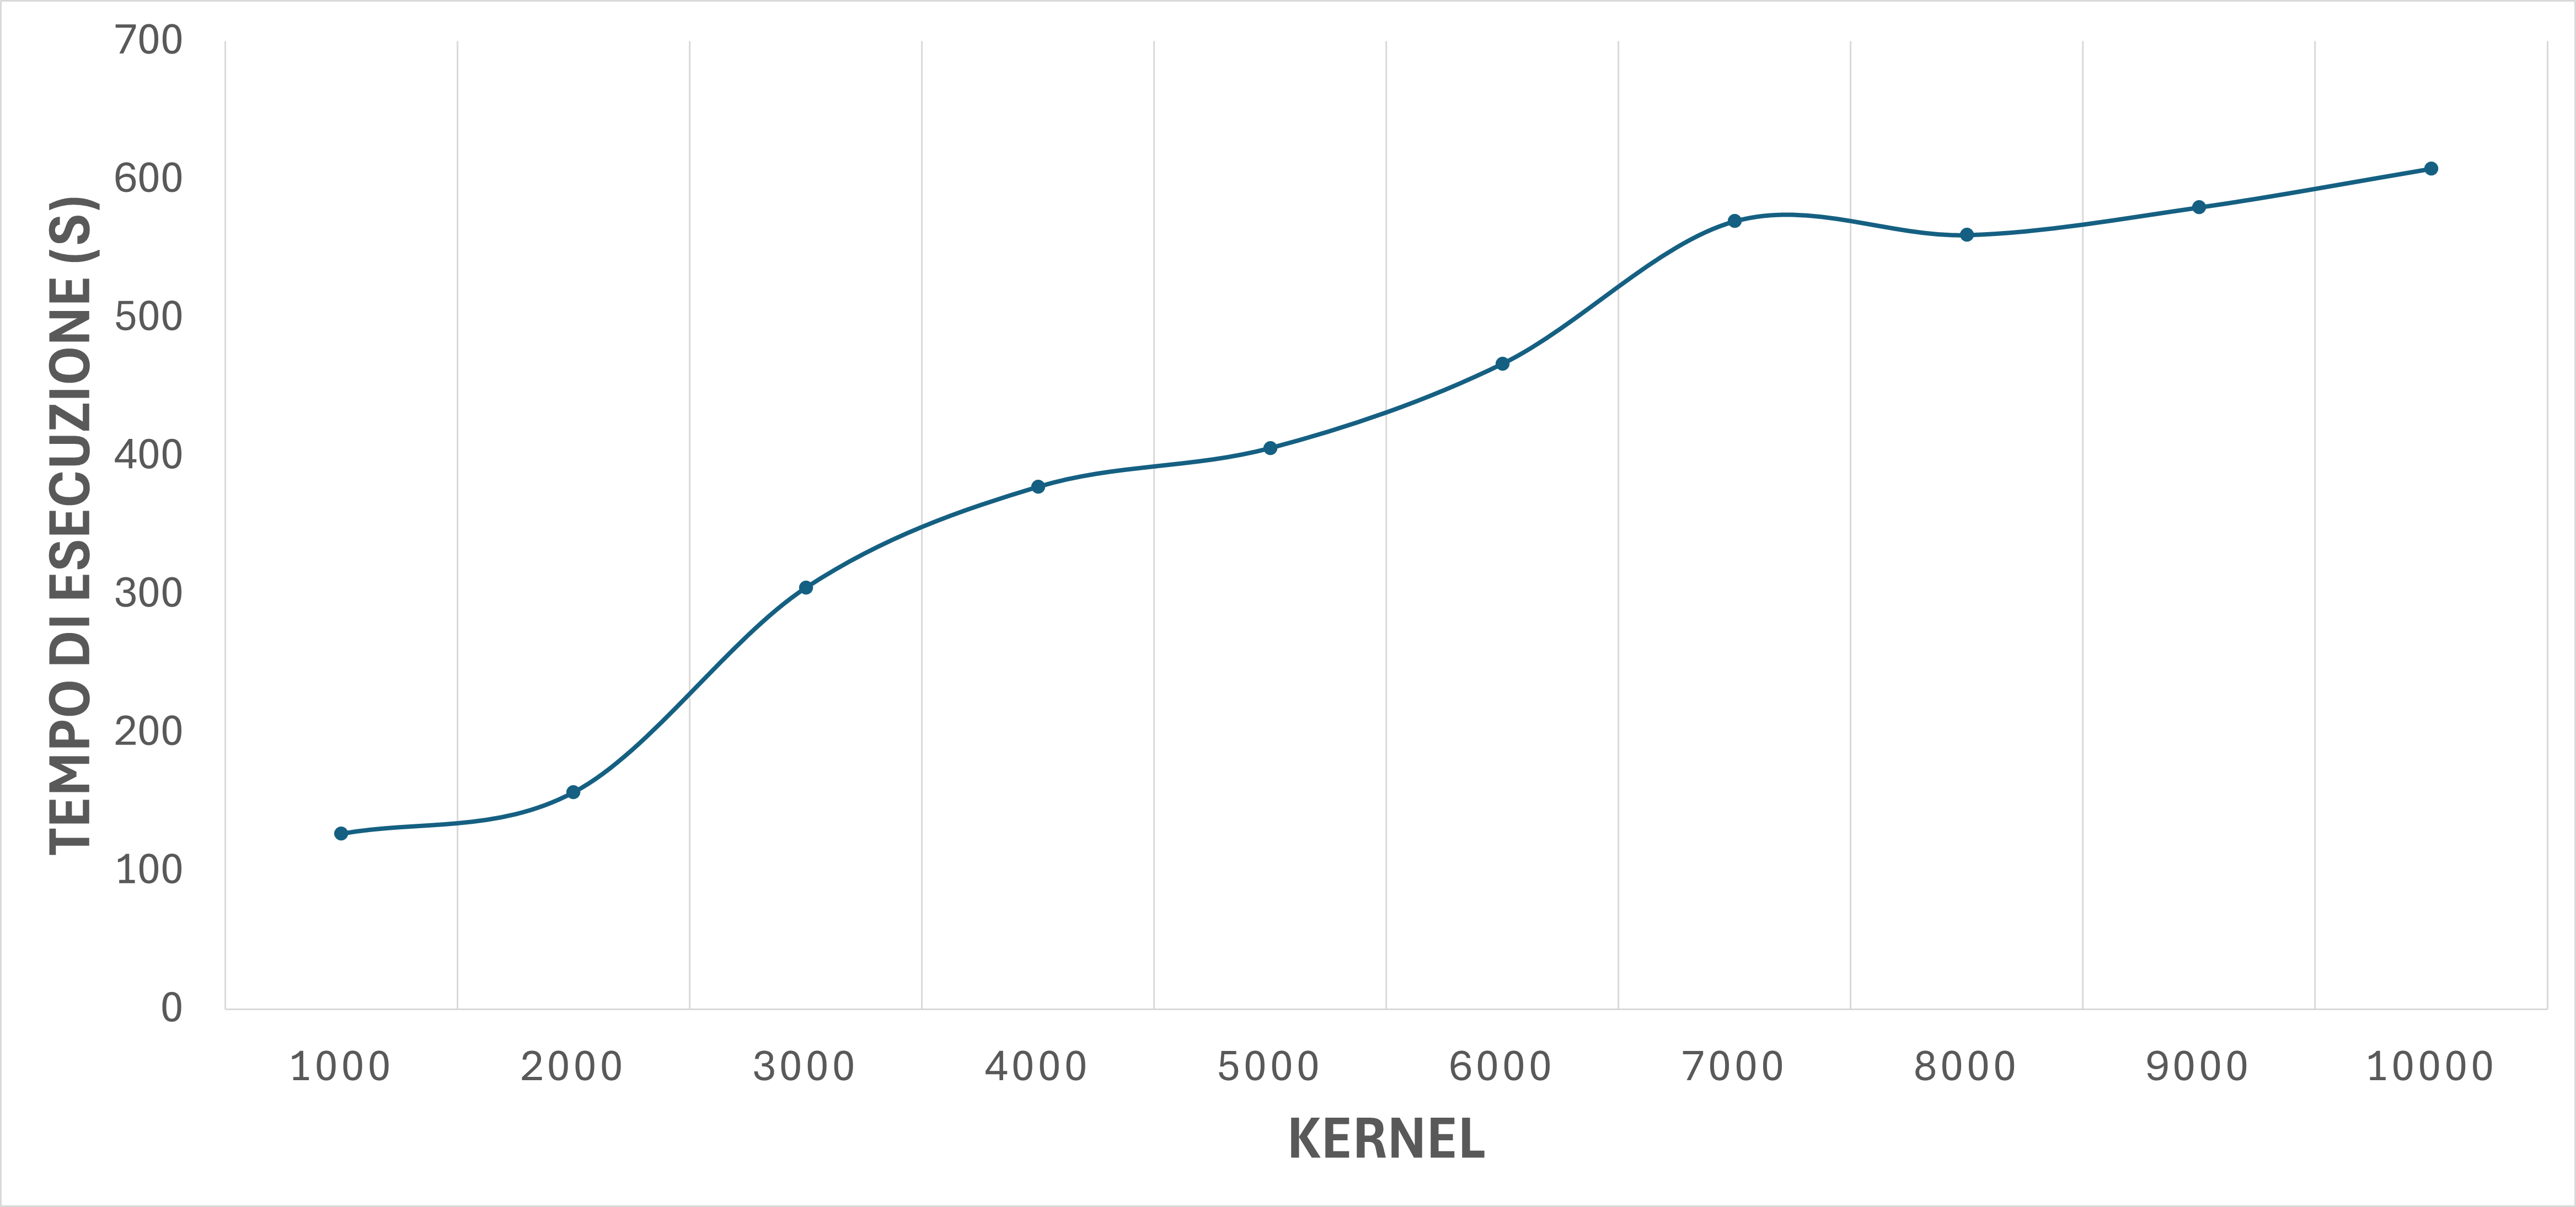
\includegraphics[width=0.9\linewidth]{images//Capitolo7/GraficoTempoEsecuzione_ROCKAD.png}
    \caption{Relazione tra Tempi di Esecuzione e Numero di Kernel}
    \label{fig:grafico_tempo_ROCKAD}
\end{figure}

Analizzando i dati raccolti fino a questo momento, ROCKET si comporta in maniera migliore in tutti i test effettuati, questo lo possiamo osservare dalle metriche, sul dataset OPS\textunderscore SAT, nelle tabelle \ref{tab:RocketOPS_SAT} e \ref{tab:ROCKAD_OPS-SAT}.
Prendendo come metrica di riferimento sempre F1, vediamo che ROCKET ottiene un punteggio di 0.797, invece ROCKAD totalizza 0.634 come picco massimo.

\section{Riflessioni}
Nonostante tutto ciò che è stato discusso precedentemente, l'utilizzo di ROCKET e ROCKAD per il rilevamento delle anomalie risulta un opzione più che valida da poter percorrere, pur rimanendo ancora troppo immatura per essere al pari di soluzioni che utilizzano modelli più comuni, i quali hanno già subito varie iterazioni di miglioramenti, come nel caso di XGBOD.

Come già evidenziato in precedenza, ROCKET e ROCKAD hanno un basso costo computazionale a confronto con modelli più complessi, questo, soprattutto nel contesto satellitare, è un punto critico a causa delle risorse hardware limitate.

ROCKET permette delle performance buone con dataset etichettati e non e potrebbe rivelarsi un buon modello per il rilevamento di anomalie.

ROCKAD, dall'altra parte, permette di essere utilizzato in un ambiente senza etichettatura dei dati e si rivela interessante per i dataset come NASA, oppure, più in generale, in un contesto reale con poche e rare anomalie, spesso non etichettate.

Purtroppo l'applicazione di ROCKAD, risulta ancora poco efficiente, dato soprattutto il suo utilizzo del modello KNN internamente, il quale porta ad una computazione maggiore ed un rischio per la scarsa capacità hardware.

\subsection{Possibili Sviluppi}
Per rendere ROCKET e ROCKAD preferibili ai già consolidati modelli, è necessario apportare ulteriori efficientamenti, così da eguagliare o addirittura superare quelli già esistenti.
Ovviamente questo serve anche per migliorare le attuali performance, già buone in alcuni campi, come l'utilizzo di ROCKET con dataset senza etichettatura.
Elenchiamo di seguito delle possibili proposte per migliorare questi modelli:
\begin{itemize}
    \item Complessità del Modello: ridurre la complessità del modello, data soprattutto dalla generazione di un gran numero di kernel e quindi di caratteristiche; questo può avvenire tramite tecniche di pruning per eliminare le caratteristiche ridondanti o non utili, riducendo la complessità del modello e la possibilità di cadere in overfitting;
    \item Compressione dei Dati: comprimere i dati permette di usarli in modo più efficiente per l'elaborazione, riducendo così anche l'uso della memoria del dispositivo satellitare;
    \item Maggiori Informazioni: data la natura casuale di ROCKET, i pattern non sono analizzabili esternamente, portando ad un limite nell'interpretazione e comprensione delle caratteristiche; migliorando questo aspetto, tramite ad esempio strumenti di visualizzazione, potrebbe portare ad un miglioramento nell'analisi dei risultati;
    \item Validazione: l'ultimo aspetto, dopo aver effettuato tutte le migliorie possibili, sarebbe l'applicazione di questi modelli in un contesto reale per validarne l'efficacia e l'efficienza, questo potrebbe avvenire, ad esempio, sulla nuova missione OPS\textunderscore SAT programmata per la fine di questo anno.
\end{itemize}
